\begin{figure}[!htb]
	\begin{center}
  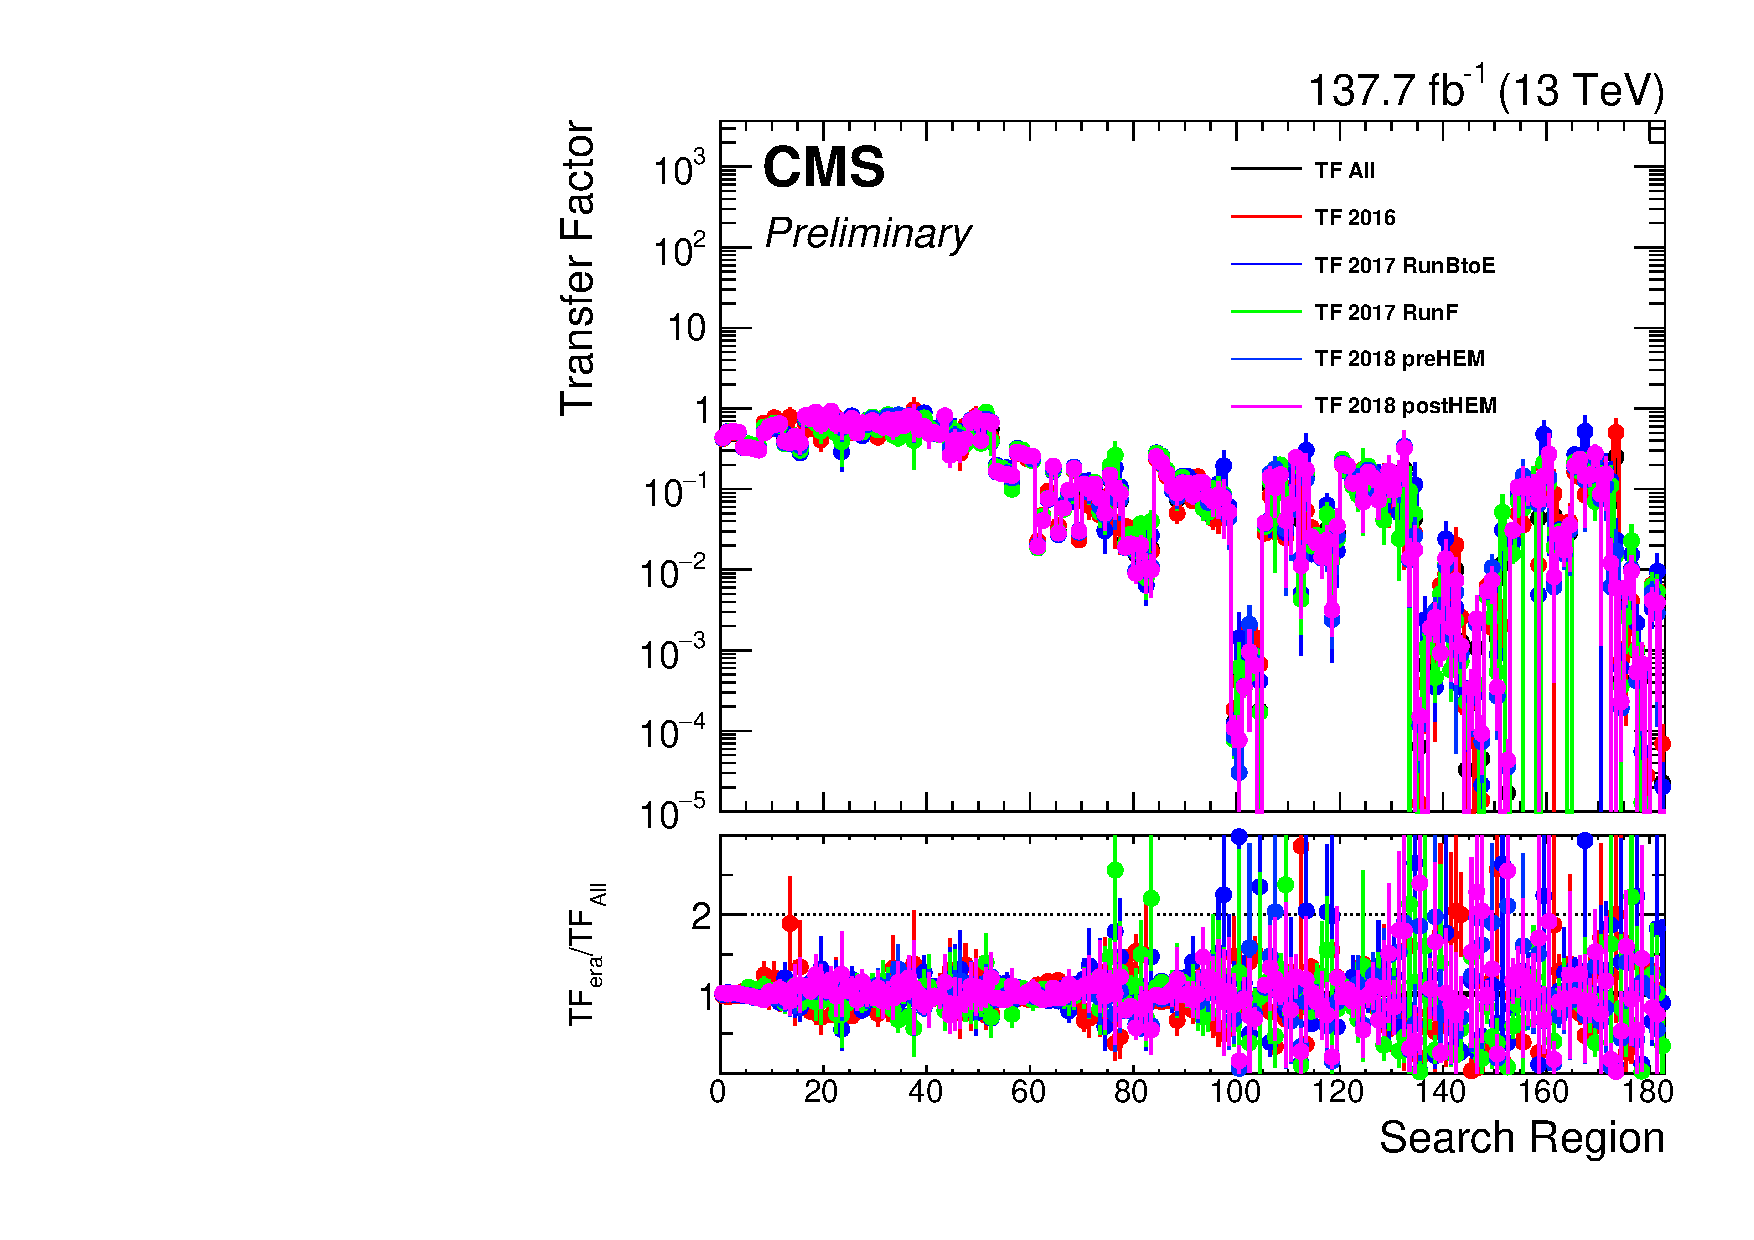
\includegraphics[width=0.4\textwidth]{LostLepton_TF_Comparison.pdf}
  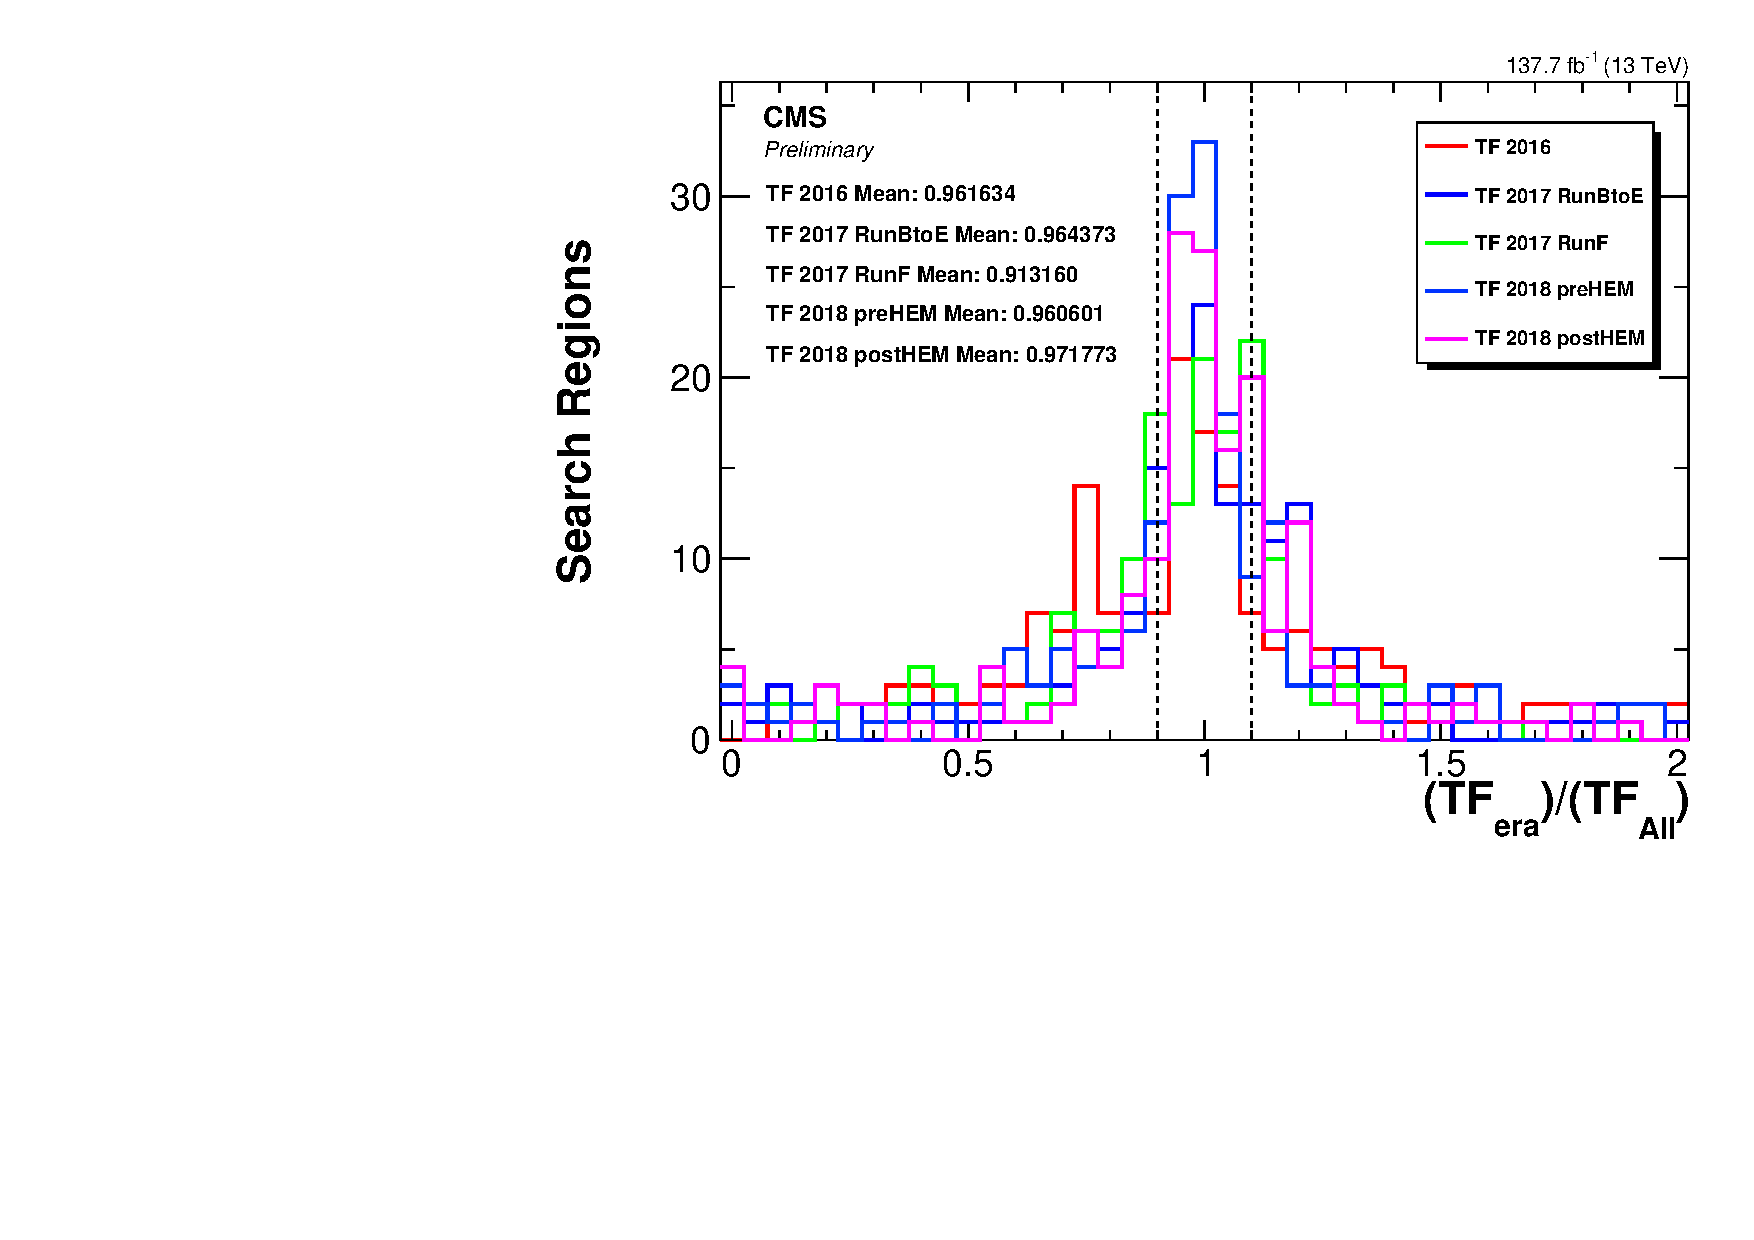
\includegraphics[width=0.5\textwidth]{LostLepton_TF_Comparison_sum.pdf} \\
	\end{center}
	\caption[Transfer Factor Comparison]{Comparisons of the transfer factors for each era of MC in the low and high \dm{} regions. The values are shown in their separate bins on the left plot and in a combined form on the right. The mean for each is also shown. 
	 }
	\label{fig:llb-1lcr-datavsmc-total-tf}
\end{figure}
\begin{figure}[!htb]
	\begin{center}  
		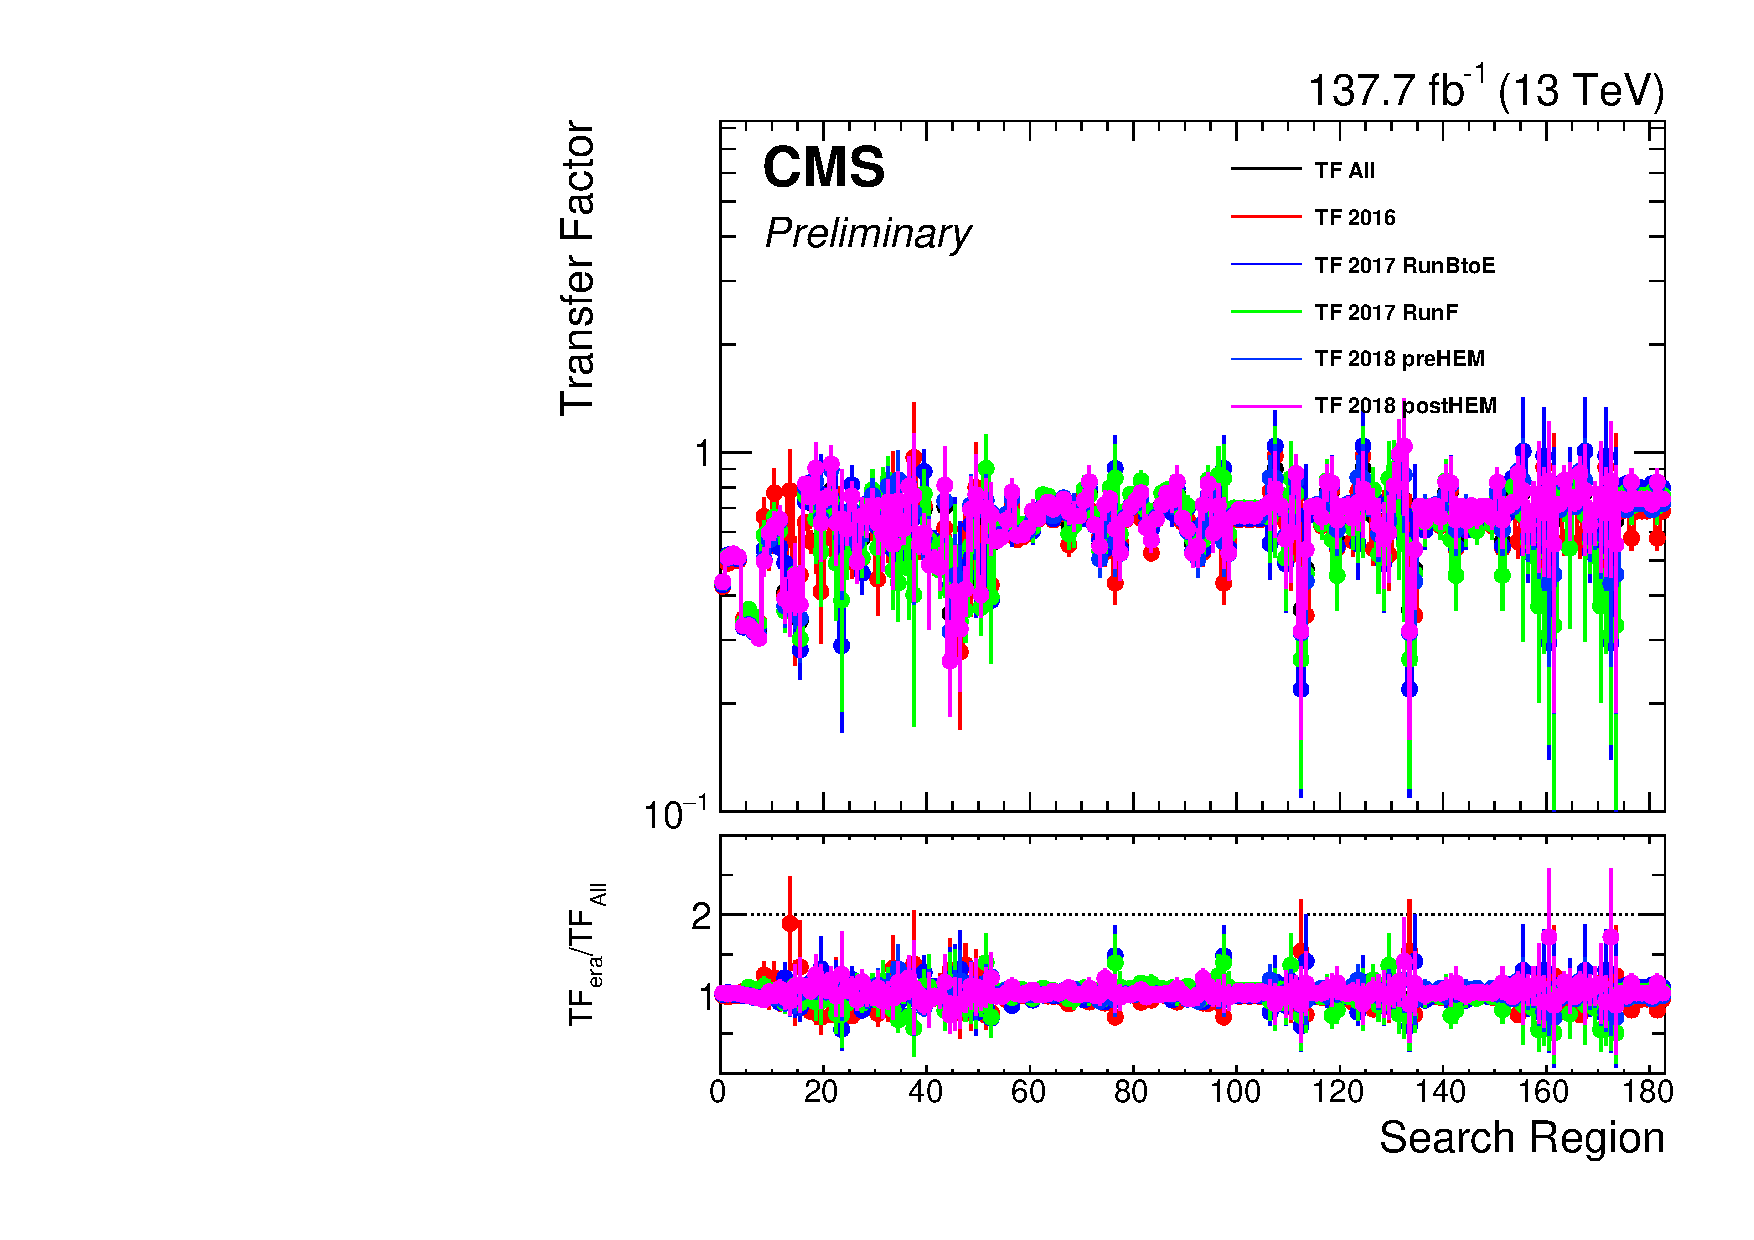
\includegraphics[width=0.4\textwidth]{LostLepton_TF_CR_to_SR_noextrap_Comparison.pdf}
		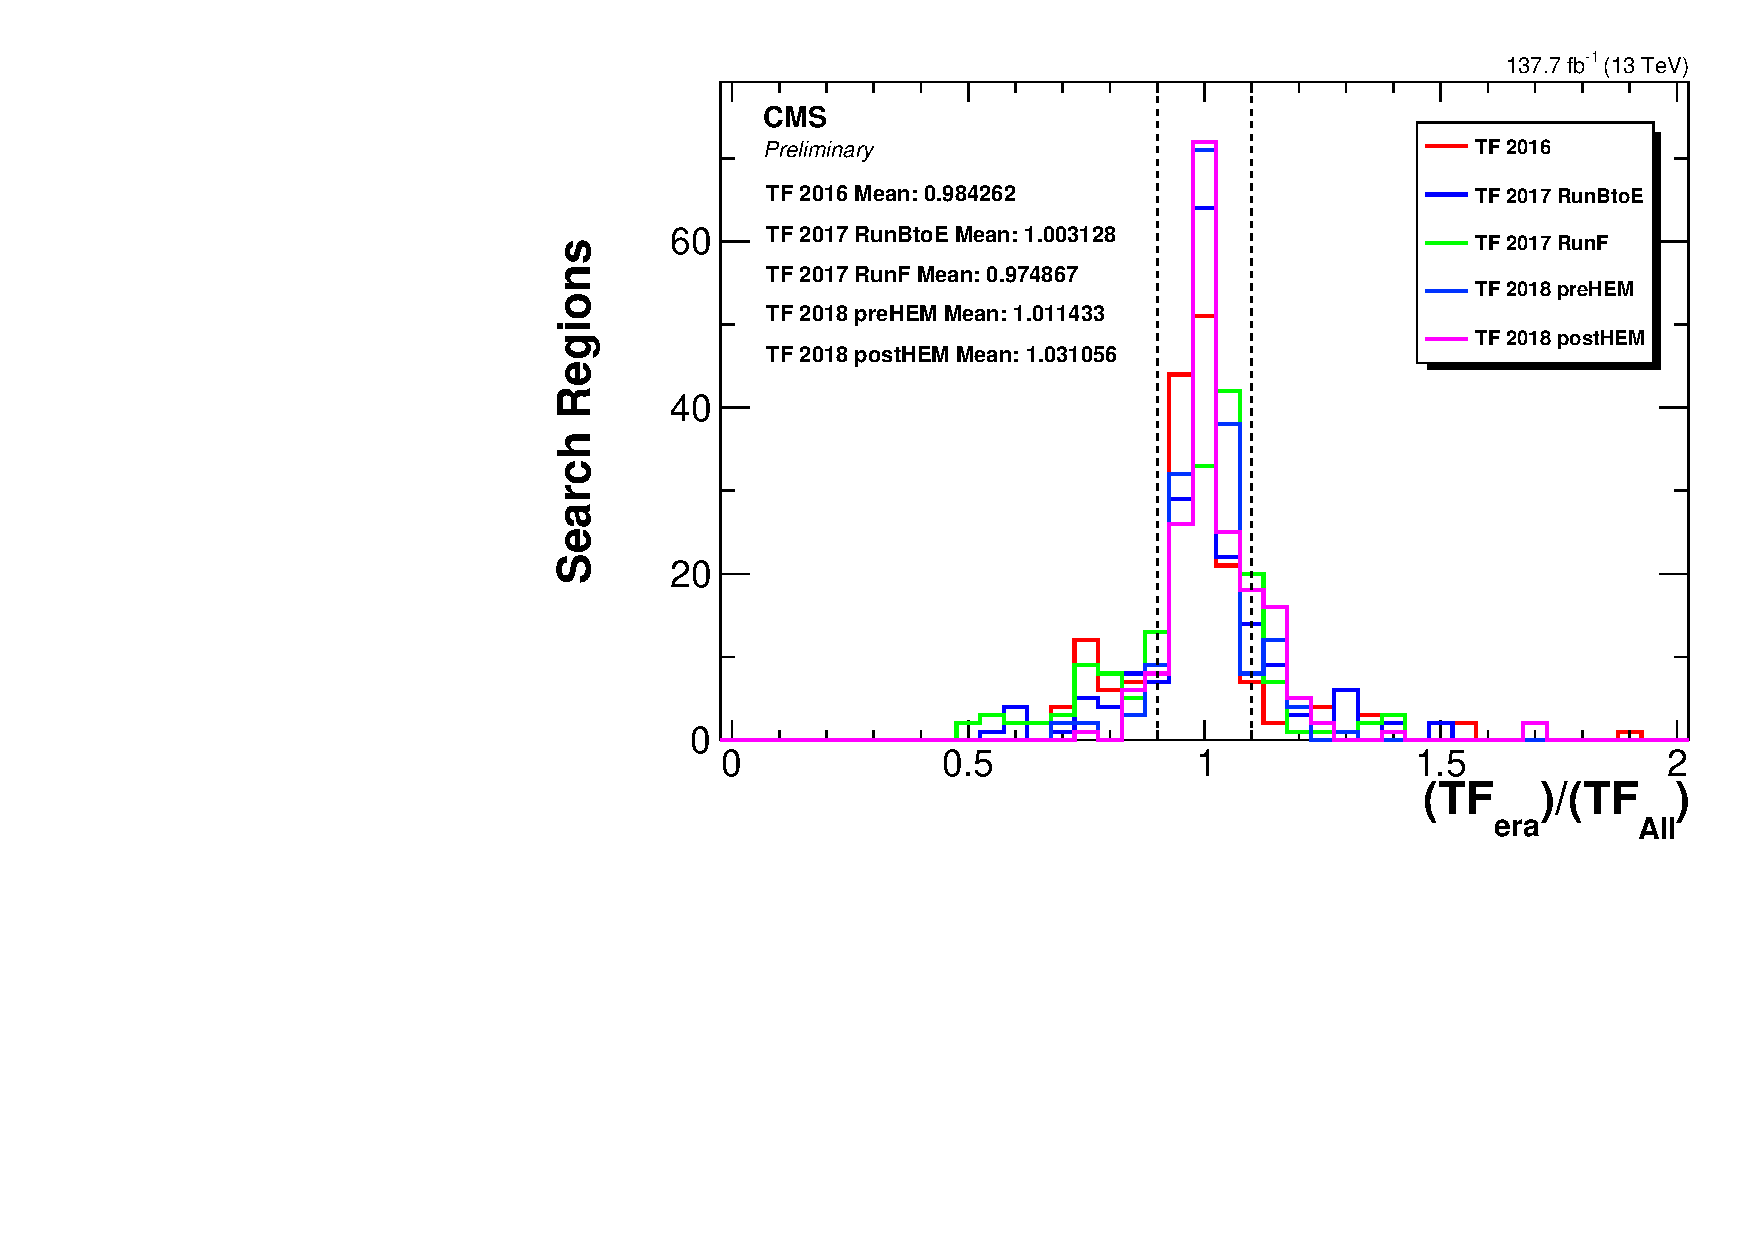
\includegraphics[width=0.5\textwidth]{LostLepton_TF_CR_to_SR_noextrap_Comparison_sum.pdf} \\
		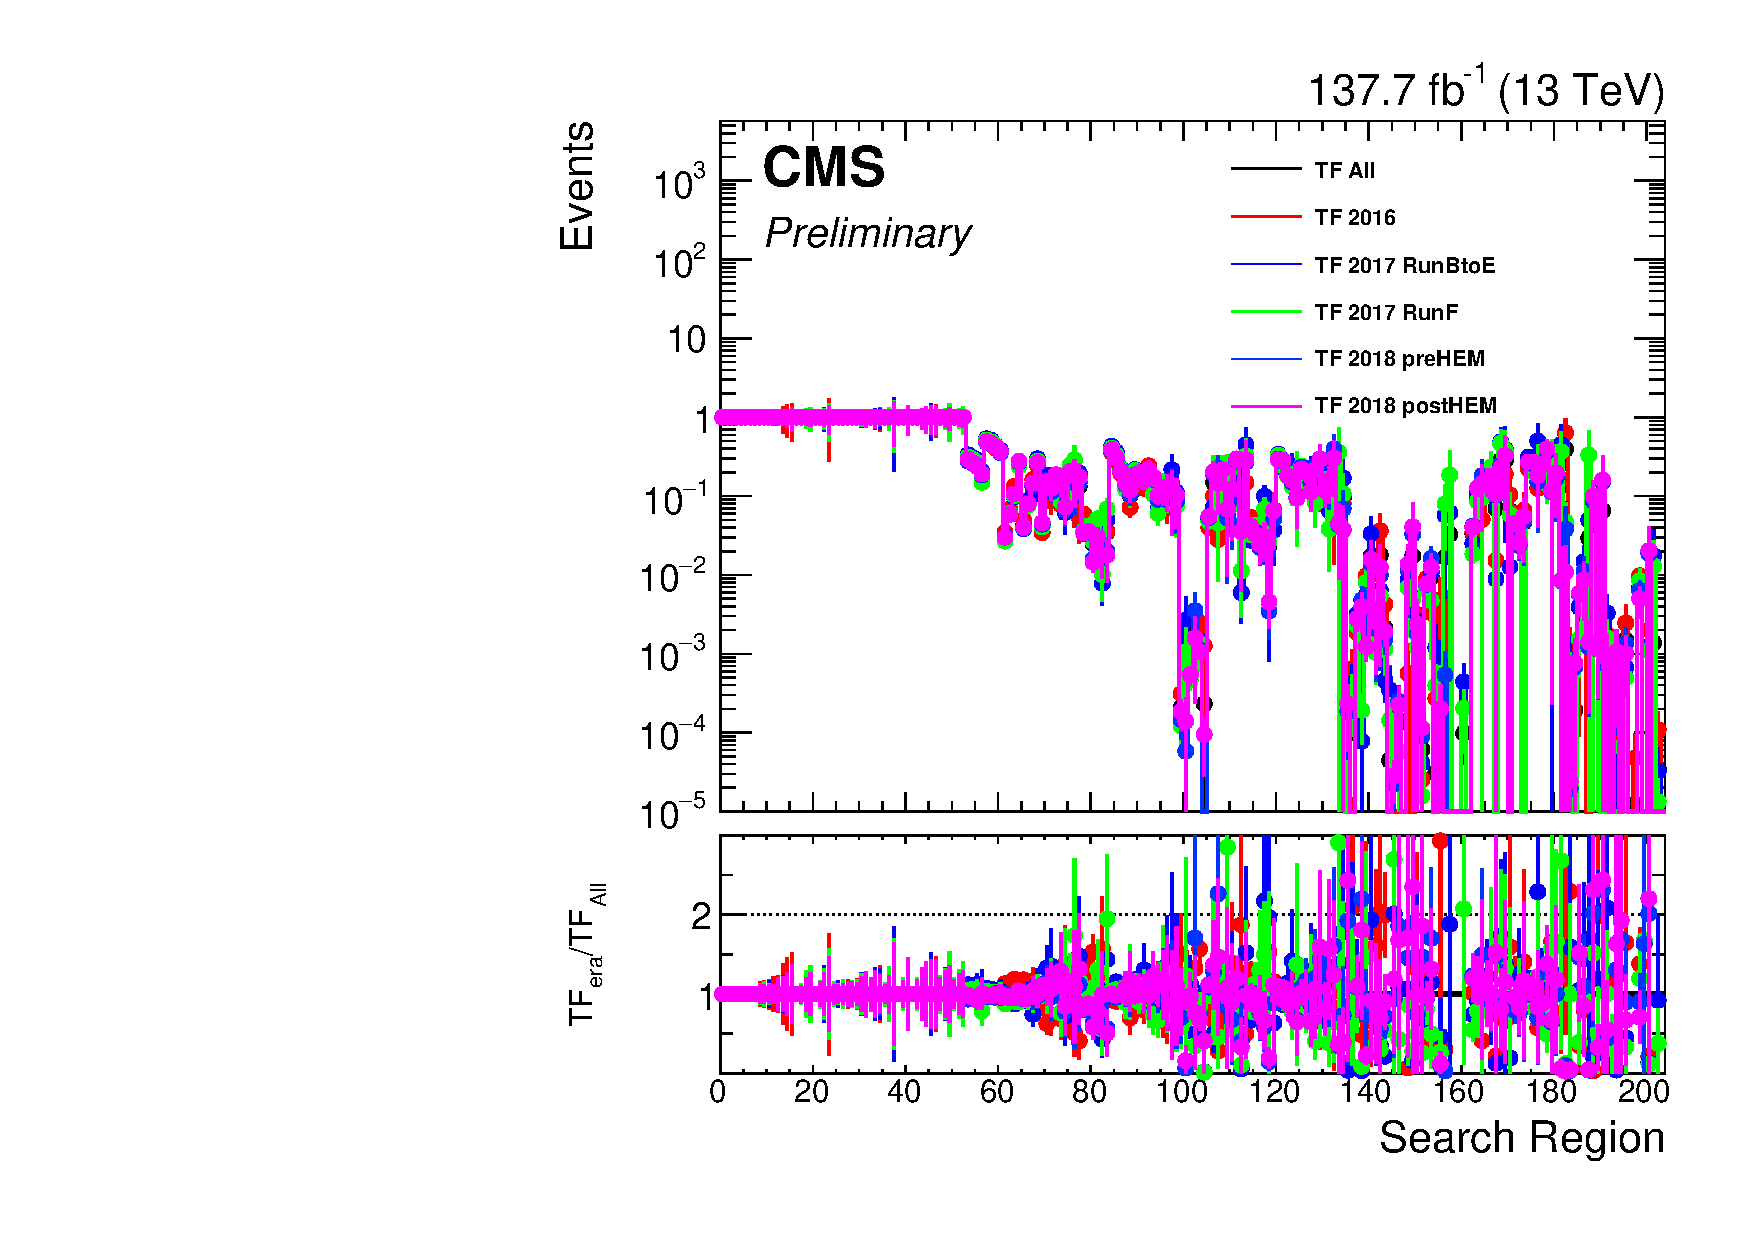
\includegraphics[width=0.4\textwidth]{LostLepton_TF_SR_extrap_Comparison.pdf}
		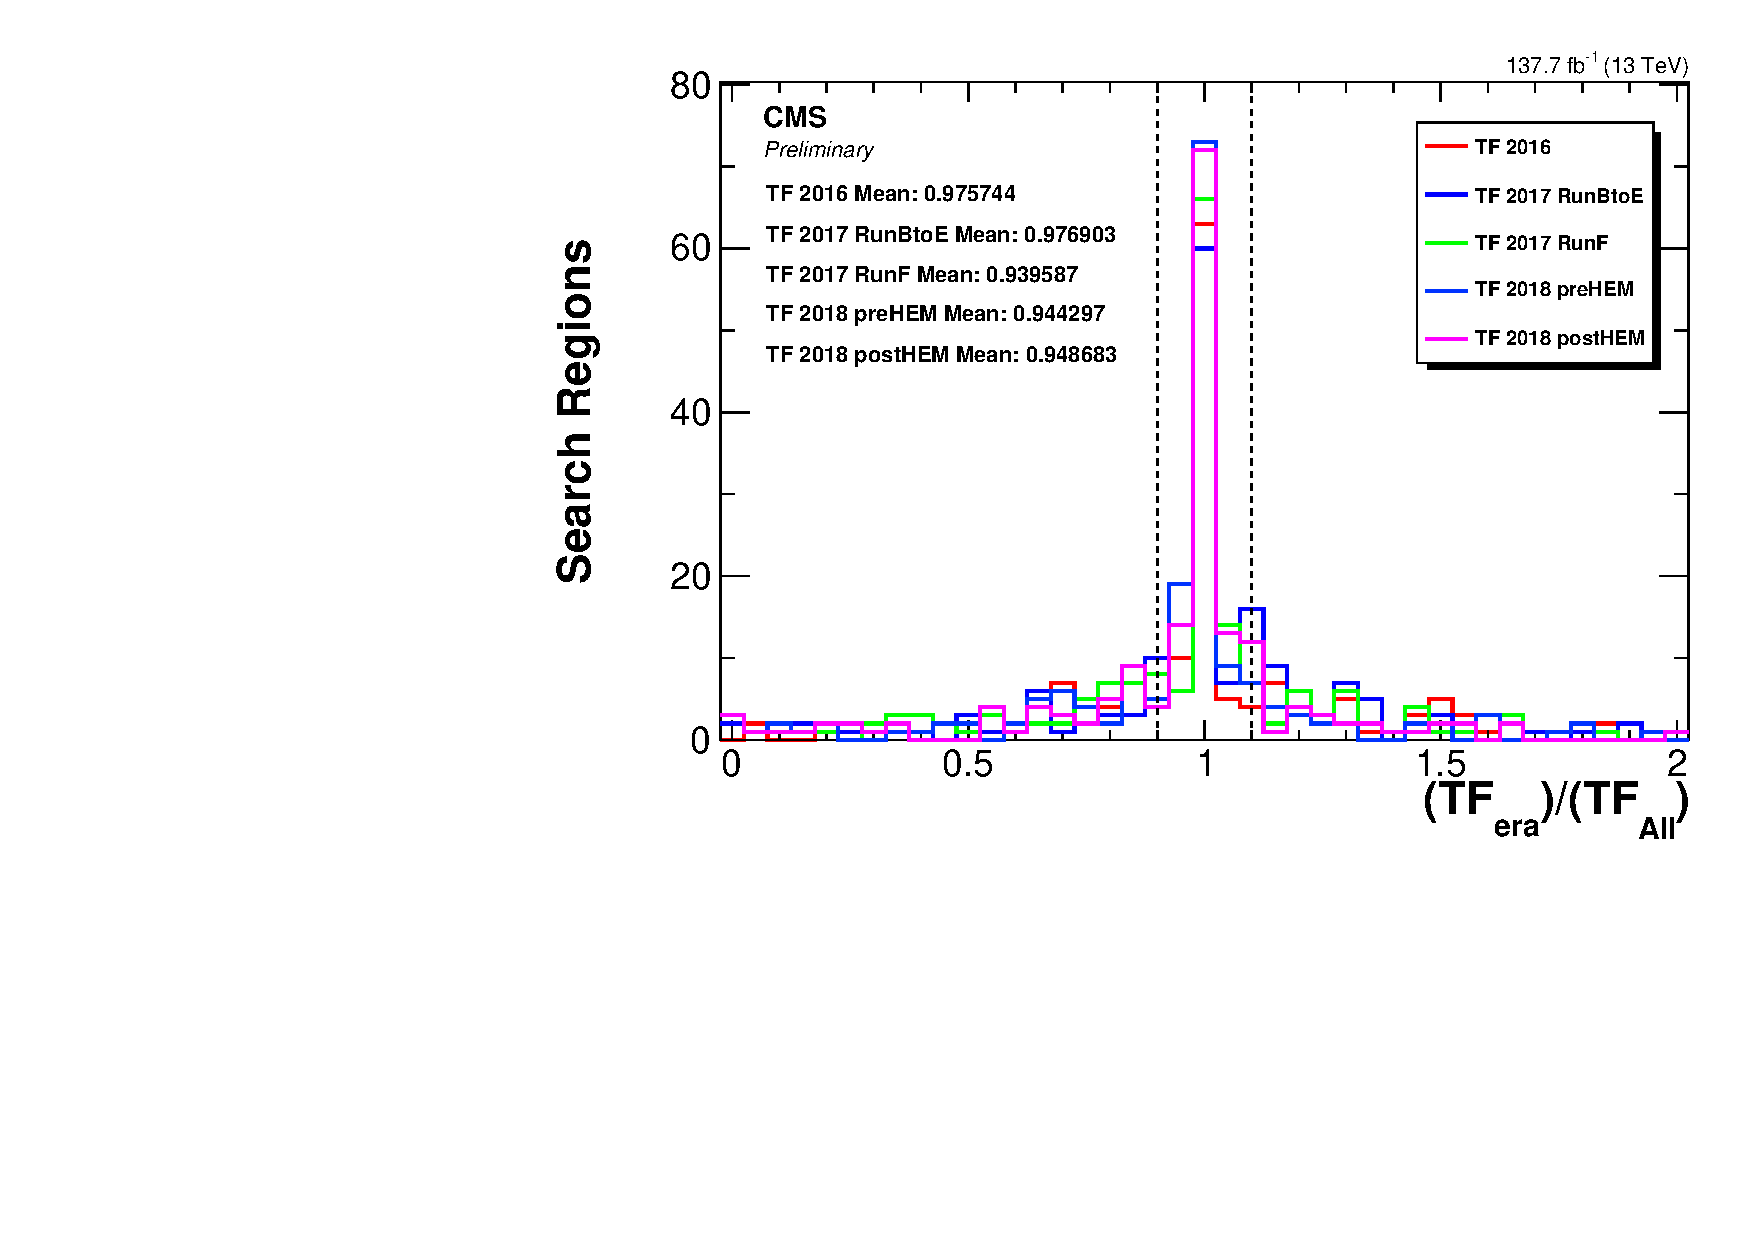
\includegraphics[width=0.5\textwidth]{LostLepton_TF_SR_extrap_Comparison_sum.pdf}
	\end{center}
	\caption[Separated Transfer Factor Comparison]{Comparisons of the transfer factors, separated into the CR-to-SR and SR-to-extrapolation, for each era of MC in the low and high \dm{} regions. The values are shown in their separate bins on the left plot and in a combined form on the right. The mean for each is also shown. 
	 }
	\label{fig:llb-1lcr-datavsmc-sep-tf}
\end{figure}
